\documentclass[11pt,a4paper,titlepage]{article}


\usepackage[utf8]{inputenc}
\usepackage[english]{babel}
%\usepackage[latin1]{inputenc}
\usepackage{amsmath}
\usepackage{amsfonts}
\usepackage{amssymb}
\usepackage{graphicx}
\usepackage{indentfirst}
\usepackage{courier}
\usepackage[nottoc,numbib]{tocbibind}
%\usepackage[colorlinks,allcolors=black]{hyperref}
\usepackage[colorlinks,allcolors=blue]{hyperref}
\usepackage{float}
\usepackage{pgfgantt}
\usepackage{lscape}
\usepackage{tabularx}
\usepackage{longtable}
\usepackage{eurosym}
\usepackage{listings}
%\usepackage{xcolor}
\usepackage{numprint}
  \npthousandsep{\,}
\usepackage{enumitem}

  
\usepackage{subfig}

\definecolor{mygray}{RGB}{245,245,245}

\definecolor{mGreen}{rgb}{0,0.6,0}
\definecolor{mGray}{rgb}{0.5,0.5,0.5}
\definecolor{mPurple}{rgb}{0.58,0,0.82}
\definecolor{backgroundColour}{rgb}{0.95,0.95,0.92}

\setlength{\parindent}{0.6cm}
\setlength{\parskip}{0.5em}
\setlength{\skip\footins}{1cm}

\author{  \LARGE Sergi Miralles Nogués }

\title{\vspace{-15mm}\textsc{\Large Facultat d'Informàtica de Barcelona (FIB)}\\\textsc{\Large Universitat Politècnica de Catalunya (UPC)\vspace{5mm}}\\\textsc{\large Grau en Enginyeria Informàtica (GEI)}\\\textsc{\large}\\{\vspace{30mm}\huge \bfseries \fontfamily{lmss}\selectfont Uptime Institute} \\ {\vspace{20mm} \LARGE \textsc{}}}
\date{19 de maig de 2020}
\begin{document}

	\maketitle
    
    \tableofcontents
    
    \newpage
    
    \section{Introducció}
    La creixent demanda en els \textit{*aaS} i l'externalització de molts components que algun dia van ser una part del nucli de les tecnologies de la informació de una empresa, com l'emmagatzemament dels documents, les còpies de seguretat, els servidors web (tant per servir al públic o per les eines d'administració per als treballadors o la intranet), així com la modernització de molts sectors que han entès que l'Internet és el present i el futur, però que no disposen dels recursos per gestionar una infraestructura que pugui oferir les prestacions que desitgen, han ajudat a crear un sector de Centres de Processament de Dades on el propietari d'aquest lloga en part o totalment, les seves maquines a aquells clients que necessitin tenir algun servei en el cloud.
    
    Per aquest motiu, els clients necessitaven obtenir garanties que el Proveïdor oferia un servei de qualitat i tot i que els SLA's ofereixen certa protecció, només s'aplica quan l'accident ja ha passat, potencialment havent interromput l'oferta dels serveis que els clients tenien hostejats en aquell CPD. Per això el 1993 Kenneth G. Brill va fundar \textbf{The Uptime Institute}, una organització centrada en el rendiment i les especificacions dels CPD's així com la seva petjada de carboni que deixen i que més tard va crear el que es coneix com \textit{Tier Standart}, una certificació que soluciona el problema mencionat anteriorment i que permet a totes les parts de un contracte per oferir serveis en un CPD extern, la seguretat que aquests podran córrer amb unes condicions de qualitat determinades. 

    
    \section{Tier Standard}
    
    L'objectiu principal del Tier Standard és avaluar de manera efectiva la infraestructura de un CPD en els requeriments d'un negoci per a la seva disponibilitat i fiabilitat i dóna una manera objectiva per comparar instal·lacions que son molt diverses. Aquesta certificació es compon de 4 nivells, anomenats \textit{Tiers}, del \textit{I} (més modest) fins al \textit{IV} (redundància completa) i mentre que els dos primers Tiers estan pensats per CPDs que no porten a càrrec tasques crítiques i que, per tant, està previst que hagin de parar les operacions per a manteniment, els dos últims Tiers proporcionen garanties de disponibilitat a través de components redundants que permeten que els negocis no quedin afectats en cas de una incidència tècnica. A més a més, aquest estàndard no pretén concretar quin tipus de components un CPD ha de tenir, ja que això mateix dificultaria la incorporació de noves tecnologies, sinó que especifica quins rols i característiques s'han d'assolir d'una manera força general. També, la certificació només s'obtindrà per aquell Tier les característiques de les quals es compleixin en la seva totalitat, per molt que una secció, important o no, de altres característiques, assoleixin requisits de Tiers superiors.
    
    L'Uptime Institute entén que un CPD no es pot operar només amb un bon disseny a la fase de l'inici del projecte i cal seguir certs protocols per assegurar la viabilitat del CPD, per això, dins de Tier Standard, proposa dues certificacions independents pero complementàries
    \subsection{Topology}
    Aquest conjunt d'especificacions és la base objectiva per a poder determinar la funcionalitat, la capacitat i la disponibilitat esperada del disseny de una instal·lació determinada en base a la configuració dels seus components. Es tenen en compte components com la refrigeració, l'alimentació, la redundància o les tasques de manteniment previstes i no previstes i el seu impacte en la infraestructura.
    \subsection{Operational Sustainability}
    Aquest conjunt de guies intenta posar a la vista els requeriments i les pràctiques en el camp de operacions que un CPD necessita per a la prevenció de caigudes dels serveis, així com les possibles respostes a esdeveniments previstos o no previstos, i es centra en les idees de que el CPD sigui gestionat per el suficient nombre de persones amb unes capacitats adients i ben entrenades, que el CPD ha de estar dissenyat per les persones i les tasques que porten a terme, a més de per les màquines, fer un ús adient dels recursos i situar el CPD en una ubicació geogràfica que no pugui portar problemes en el futur, i si els porta, que aquests estiguin planejats
    
    \section{Tiers}
    Els dos primers Tiers, I i II, estan orientats a operacions que busquen com a objectiu un desplegament ràpid i barat i que no ofereixen un producte que és molt sensible a fallades en la disponibilitat sistema. Per altra banda, els Tiers III i IV estan més orientats a aquelles operacions que el seu objectiu principal és la disponibilitat i la fiabilitat dels seus serveis i permeten als operadors d'aquests serveis escalar amb relativa facilitat i sense disrupcions del sistema significatives.
    
    Una característica clau dels requisits és que aquests no especifiquen cap referència absoluta o mida concreta com ara \textit{Nombre de unitats d'aire condicionat} i, en el cas de un CPD qualsevol de Tier II, es podria dividir la seva capacitat en dos i utilitzar aquests components sobrants per oferir redundància, i així complir amb molts dels requisits que un Tier III ens demana.
    
    Com és d'esperar, els requisits per obtenir un Tier son acumulatius, el que significa que per obtenir el Tier \textit{N+1} cal haver superat tots els requisits per el Tier \textit{N}. Per això, en aquesta secció només es mencionaran les característiques que diferencien el Tier tractat respecte l'anterior.
    
\begin{figure}[h]
    \centering
    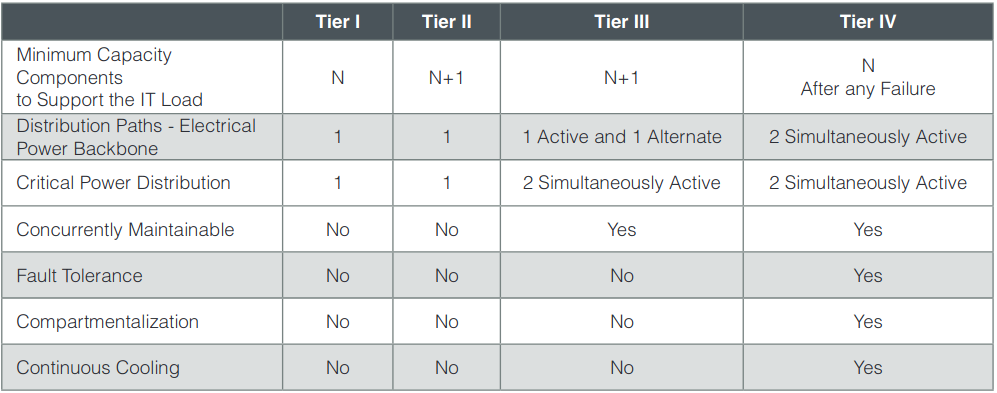
\includegraphics[width=12cm]{Tier requirement list.png}
    \caption{Taula bàsica de les prestacions de cada Tier}
    \label{fig:Tier_req_sum}
\end{figure}
    
    \subsection{Tier I. Basic Site Infrastructure}
    Aquest Tier satisfà les demandes bàsiques per a poder tenir una infraestructura dedicada al servei de sistemes de les TI. Aquest Tier proporciona unes característiques millorades respecte a una possible sol·lució a la mateixa oficina i disposa de components bàsics com un SAI, refrigeració o un generador per emergències.
    %Necessitat d'aturada completa del sistema per efectuar tasques de manteniment o reparació. La instal·lació és completament vulnerable a fallades de components.
    
    \subsubsection{Requeriments fonamentals}
    \begin{enumerate}[nolistsep, label=\alph*.]
    \item Espai dedicat per sistemes de gestió, SAI, sistema de refrigeració per la sala de ordinadors i sistema de generació de electricitat per emergències
    \item 12h de combustible per generar electricitat
    \end{enumerate}
    
    \subsubsection{Tests de confirmació}
    \begin{enumerate}[nolistsep, label=\alph*.]
    \item Hi ha capacitat suficient per a cobrir les necessitats de les operacions.
    \item El manteniment requerirà que tot o gairebé totes les instal·lacions quedin aturades
    \end{enumerate}
    
    \subsubsection{Impactes en la Operació}
    \begin{enumerate}[nolistsep, label=\alph*.]
    \item Activitats planejades i no planejades interrumpiran l'operació del sistema, així com alguns errors humans
    \item La fallada de qualsevol component impactarà en l'estabilitat del sistema
    \item La instal·lació es pararà completament un cop a l'any per efectuar tasques de manteniment, tot i que pot ser més sovint en casos necessaris
    \end{enumerate}
    
    \subsubsection{Operational Sustainability}
    \begin{enumerate}[nolistsep, label=\alph*.]
    \item Hi ha personal amb les qualificacions necessàries assignat al manteniment actiu
    \item Polítiques de manteniment que permeten tenir traçabilitat i seguiment dels problemes
    \item Documentació sobre l'edifici i els seus entorns així com els components que integren el CPD
    \end{enumerate}
    
    
    
    \subsection{Tier II. Redundant Site Infrastructure Capacity Components}
    Aquest Tier disposa de redundància en els sectors més crítics de un CPD i proporcionen una major seguretat contra a fallades dels components. Aquests pertanyen al rol de la refrigeració i del subministrament d'energia. De totes maneres, una averia o una tasca de manteniment pot obligar a parar tot o part de les operacions.
    %Disposa d'alguns components redundants pero continua sent necessari apagar les maquines per efectuar manteniment.
    
    \subsubsection{Requeriments fonamentals}
    \begin{enumerate}[nolistsep, label=\alph*.]
    \item Es disposa dels següents components de forma redundant: Generador d'electricitat i tanc de combustible, SAI i sistema de refrigeració.
    \end{enumerate}
    
    \subsubsection{Tests de confirmació}
    \begin{enumerate}[nolistsep, label=\alph*.]
    \item Els elements redundants es poden treure del servei sempre que s'hagi establert amb antelació sense haver d'aturar les operacions que s'estan duent a terme en la resta de les instal·lacions
    \item Tots els elements redundants poden ser aturats (per manteniment, per exemple) sense haver d'aturar les operacions.
    \end{enumerate}
    
    \subsubsection{Impactes en la Operació}
    \begin{enumerate}[nolistsep, label=\alph*.]
    \item La instal·lació no es pot aturar per manteniments
    \item La deixada de funcionament d'algun dels components pot afectar al funcionament del CPD
    \end{enumerate}
    
    \subsubsection{Operational Sustainability}
    \begin{enumerate}[nolistsep, label=\alph*.]
    \item Es manté una millor traça dels problemes i com s'han implementat les sol·lucions
    \item Es disposa de suport d'experts de les empreses dels components que integren el sistema a l'abast
    \item Es manté una millor higiene
    \item Es disposa de documentació explicant les operacions que es porten a terme i perquè així com plans de mitigació de riscos
    \item Es comproven regularment els plans de la sala d'ordinadors en busca de reestructuracions
    \item S'assegura que la càrrega màxima no excedeix el seu disseny inicial i que els sistemes redundants no son necessaris per suportar aquesta càrrega
    \item Control i aplicació de paràmetres ambientals com Temperatura, Humitat o Volum d'aire.
    \item Espai dedicat a l'emmagatzemament de recanvis i al muntatge i prova d'aquests
    \item Seguretat a nivell de sales d'ordinadors i zones crítiques de suport
    \end{enumerate}
    
    \subsection{Tier III: Concurrently Maintainable Site Infrastructure}
    Aquest Tier ja és més apte per a desplegaments crítics i introdueix el concepte de \textit{Concurrent Maintainance},  que consisteix en la possibilitat, tal i com indica el nom, efectuar tasques \textbf{planejades} de manteniment o millora sense que CPD pateixi cap mena de impacte en el seu rendiment. Per aquest motiu tots els components han d'estar replicats per poder ser posats fora de línia i hi ha d'haver dos camins diferents de electricitat i refrigeració que arribin a cada rack. Per descomptat, el concepte de Concurrent Maintainance també aplica a aquells sistemes més apartats de la operació principal del CPD, per exemple motors de la cel·lula elèctrica o els controladors de una AE\footnote{Apagada d'Emergència}.
    %Cada component disposa de una alternativa redundant que evita que la instal·lació deixi de funcionar en cas de manteniment. Tot i així, fallades no previstes poden obligar a parar les operacions.
    \newpage
    \subsubsection{Requeriments fonamentals}
    \begin{enumerate}[nolistsep, label=\alph*.]
    \item Sistema de ventilació i subministrament intern d'electricitat completament redundant.
    \item Tots els components disposen de dos fonts d'alimentació
    \item El motor de la cel·lula de generació d'electricitat no té restriccions d'ús continu
    \end{enumerate}
    
    \subsubsection{Tests de confirmació}
    \begin{enumerate}[nolistsep, label=\alph*.]
    \item Qualsevol component pot ser tret de servei sense perjudicar el rendiment del sistema.
    \end{enumerate}
    
    \subsubsection{Impactes en la Operació}
    \begin{enumerate}[nolistsep, label=\alph*.]
    \item Es poden utilitzar els sistemes redundants per a realitzar operacions de manteniment sense afectar a les operacions del sistema
    \item El CPD és més vulnerable quan els sistemes redundants s'estan fent servir a causa de un exercici de manteniment
    \item Com que el sistema de subministrament elèctric només té una presa de corrent a l'exterior, la instal·lació encara és vulnerable a interrupcions no planejades del sistema
    \end{enumerate}
    
    \subsubsection{Operational Sustainability}
    \begin{enumerate}[nolistsep, label=\alph*.]
    \item Presencia mínima de una persona qualificada en tot moment en les instal·lacions
    \item Disponibilitat d'equips especialitzats en els diversos components del CPD
    \item Documentació i traçabilitat en el manteniment i substitució dels sistemes redundants i la avaluació posterior de la efectivitat d'aquestes operacions
    \item Programa de manteniment i prevenció efectiu
    \item Programes específics de formació per els empleats
    \item Monitorització i previsió del consum d'electricitat, espai utilitzat i refrigeració necessària
    \item Propòsit clar del CPD en el seu disseny
    \item Espais separats de la sala d'ordinadors per dur a terme tasques de gestió, manteniment, emmagatzematge o training així com distancia suficient de l'edifici respecte les parcel·les adjacents per evitar possibles accidents
    \item Control d'accés a l'edifici i revisions periòdiques de les polítiques de seguretat
    \item Flexibilitat per incrementar la capacitat del CPD i una infraestructura que permeti desenvolupar les operacions així com el manteniment més fàcilment.
    \end{enumerate}
    
    
    
    \subsection{Tier IV: Fault Tolerant Site Infrastructure}
    A més a més de poder realitzar operacions de manteniment planejades, aquest Tier permet que totes les operacions no siguin afectades si falla qualsevol component (i per tant, tots els components que depenen directament de ell), en qualsevol moment
    %Una fallada individual de qualsevol component no obligarà a l'aturada del CPD i aquest es podrà mantenir operacional durant varies hores
    
   \subsubsection{Requeriments fonamentals}
    \begin{enumerate}[nolistsep, label=\alph*.]
    \item Tots els sistemes replicats en espais diferents de l'edifici i camins diferents per components com l'electricitat o la refrigeració
    \item Tots els sistemes de distribució han d'estar compartimentats per evitar possibles afectacions de un sistema que falla cap a l'altre
    
    \end{enumerate}
    
    \subsubsection{Tests de confirmació}
    \begin{enumerate}[nolistsep, label=\alph*.]
    \item La fallada de qualsevol component no afectarà a l'operativitat del sistema
    \item Hi ha un traspas autònom de recursos quan algun d'aquest falla cap a la seva replica
    \item Es poden extreure tots els  components sense afectar a les operacions
    \end{enumerate}
    
    \subsubsection{Impactes en la Operació}
    \begin{enumerate}[nolistsep, label=\alph*.]
    \item La instal·lació no és vulnerable a fallades sobtades de cap component
    \end{enumerate}
    
    \subsubsection{Operational Sustainability}
    \begin{enumerate}[nolistsep, label=\alph*.]
    \item CC\footnote{Continuous Cooling. Sistema que permet no entrar en una situació en que tot l'equipament que genera calor funciona mentre que el sistema de refrigeració ha deixat de funcionar} és obligatori
    \end{enumerate}
    
    \newpage
\section{Bibliografia}
    
    
    \begin{itemize} 
    \item \href{https://uptimeinstitute.com/uptime_assets/889d381be3ad2900e838d497ba1ed0a2dbda4bbd31454b2d475eb986f2af3a55-00001E.pdf}{chl.li/OnZxV}
    \item \href{https://uptimeinstitute.com/uptime_assets/2f9322a6147d57500439cc472a8e26b9339e1142f707dd70ef43817a78359041-00002A.pdf}{chl.li/5kY71}
    \item \href{https://uptimeinstitute.com/images/award-terms-and-conditions/UIPS_SCHEDULE-I-TC_Tier-and-Operational-Sustainability-Certification-Terms-and-Limitations_150701-2935C.pdf}{chl.li/GE2HZ}
    \item \href{https://journal.uptimeinstitute.com/explaining-uptime-institutes-tier-classification-system/}{chl.li/gGysL}
    \item \href{https://www.datacenterknowledge.com/archives/2009/10/23/the-uptime-institute-sold-to-451-group}{chl.li/G0s5Z}
    \item \href{https://www.spglobal.com/marketintelligence/en/media-center/press-release/sp-global-acquires-451-research-llc}{chl.li/zb6YV}
    \item \href{https://web.archive.org/web/20150521015255/http://www.redlands.edu/7231.aspx}{chl.li/gtDKE}
    \item \href{https://download.schneider-electric.com/files?p_Doc_Ref=SPD_ASTE-5T3TTT_EN}{chl.li/OVsAJ}
    \item \href{https://wilsonengineered.com/Tech/TUI809ContinuousCooling_WP.pdf}{chl.li/wnlAh}
    \end{itemize}

 


\end{document}
